\documentclass[11pt]{article}
\usepackage[utf8]{inputenc}
\usepackage{amsmath}
\usepackage{amsfonts}
\usepackage{amssymb}
\usepackage{bm}
\usepackage{geometry}
\usepackage{xcolor}
\usepackage{tikz}
\usepackage{hyperref}

\geometry{margin=1in}

\title{Unpenalized Magnitude Recovery for Signed Biological Networks\\
\large Stage (c): De-biased Refit via Bound-Constrained Optimization}
\author{Algorithm Specification}
\date{\today}

\begin{document}

\maketitle

\begin{abstract}
This document specifies a follow-on ``Stage (c)'' algorithm designed to recover unbiased edge magnitudes in a multi-state Poisson GLM for spiking neural networks. While the preceding EM-FDR-Bagging stage robustly identifies the topological support of the network (detecting true edges and assigning Dale's principle signs), its use of $L_1$ regularization systematically shrinks edge magnitudes. In addition, repeated enforcement of a spectral-radius bound can further scale down the fitted connectivity matrix when the unconstrained update would exceed the stability limit. To isolate magnitude estimation from structural discovery, we define a bound-constrained optimization task that freezes the discovered topological mask, removes the sparsity penalty, and enforces biological signs. The recommended implementation fits compact active-parameter vectors rather than dense mostly-zero matrices: signed Dale-constrained entries are represented by squared parameters, free entries are copied directly, and the full matrix $A$ is rebuilt in the forward pass.
\end{abstract}

% ===============================================================
\section{Introduction and Background}
% ===============================================================

The full analysis pipeline is organized into three stages. \textbf{Stage (a)}
is the ordinary PRISM-EM fit on the chosen spike-train window: it estimates a
shared connectivity matrix, state-dependent biases, and a reference decoded
state sequence; this core fitter is specified in
\texttt{fitEM\_states\_ver3c.tex}. \textbf{Stage (b)} is the
EM-FDR-Bagging procedure specified in
\texttt{fitFDR\_states\_ver3c.tex}: it reuses the Stage (a) reference state
labels, performs bagged locked M-step refits, calibrates edges against
time-scrambled null fits, and returns a statistically vetted support mask
with conservative edge magnitudes. \textbf{Stage (c)} is the de-biased
refit described in this document: it freezes the Stage (b) support and
Dale-sign decisions, removes the \(L_1\) sparsity penalty, and refits final
edge magnitudes and state biases under the remaining biological and
stability constraints.

\subsection{Input Data and Model Summary}
The input consists of a discrete spike-train recording of $N$ neurons over $T$ time bins of width $\Delta t$, yielding a count matrix $Y \in \mathbb{R}^{T \times N}$. The system is modeled as a non-stationary, multi-state Poisson Generalized Linear Model (GLM). The conditional firing rate for neuron $i$ at time $t$ depends on a shared connectivity matrix $A \in \mathbb{R}^{N \times N}$ and a state-dependent bias vector $B_{\hat{S}_t}$:
\begin{equation}
\label{eq:model-rate}
\lambda_t = \exp\big(\min(A Y_{t-1} + B_{\hat{S}_t},\ \eta_{\text{clip}})\big)\,\Delta t, \qquad Y_t \sim \text{Poisson}(\lambda_t)
\end{equation}
where $\hat{S}_{1:T}$ is the hard-decoded state sequence used by the M-step, and $\eta_{\text{clip}}$ prevents numerical overflow. In locked mode $\hat{S}_{1:T}$ is copied from Stage (b); in refit mode it is updated by the Stage (c) E-step and Viterbi decode before the following de-biased M-step.

\subsection{The Preceding FDR-Bagging Stage}
Prior to this stage, an EM-FDR-Bagging routine was run. It drew subsamples of lag pairs and fit the model using an $L_1$ penalty (Lasso shrinkage) to suppress noise. Edges that survived a source-pooled null hypothesis across multiple bags were retained. Furthermore, source neurons were classified based on their total outgoing edge sum: strictly positive columns were labeled Excitatory, strictly negative columns were labeled Inhibitory, and intermediate columns were labeled Undecided.

The output of the bagging stage provides:
\begin{enumerate}
    \item A vetted topological mask indicating which edges are statistically significant.
    \item A categorical label for each source node: \texttt{Excitatory}, \texttt{Inhibitory}, or \texttt{Undecided}.
    \item Approximate, heavily $L_1$-shrunk point estimates for the connectivity ($\bar{A}$) and state biases ($\bar{B}$).
\end{enumerate}

% ===============================================================
\section{Motivation: The Need for a De-biased Refit}
% ===============================================================

Because the FDR-Bagging stage relies on an $L_1$ penalty to identify structural zeros, all surviving non-zero edges in $\bar{A}$ are systematically biased toward zero. This is a well-known property of Lasso regression. The shrinkage is useful during edge discovery because it suppresses noisy weak coefficients, but it is undesirable once the support has already been selected.

There is a second, model-specific source of underestimation. PRISM-EM also enforces a spectral-radius limit, $\rho(A)\le\rho_{\text{max}}$, to keep the recurrent GLM numerically stable. If an M-step update produces a matrix with $\rho(A)>\rho_{\text{max}}$, the projection rescales the effective matrix. This operation preserves the discovered edge pattern and signs, but it can reduce many edge magnitudes at once. Therefore, the Stage (b) aggregate $\bar{A}$ should be interpreted as a conservative, regularized support estimate, not as a final magnitude estimate.

To recover the biological magnitudes of these connections, we perform a ``de-biased Lasso'' step: an unpenalized Maximum Likelihood Estimation (MLE) refit restricted to the selected topological support. The simplest mode keeps the Stage (b) state sequence locked, matching the FDR-bagging refits; the multi-state mode may instead alternate de-biased M-steps with state refitting.

The state biases should be re-fitted in the same optimization. In Eq.~\eqref{eq:model-rate}, $A Y_{t-1}$ and $B_{\hat{S}_t}$ enter the log-rate additively, so residual coupling between the connectivity and the state-dependent baseline can remain after the support-discovery stage. Once the magnitudes in $A$ are allowed to expand without the $L_1$ penalty, the optimum values of $B$ may also shift.

This is a bound-constrained optimization problem. We must maximize the Poisson log-likelihood while enforcing four strict rules:
\begin{enumerate}
    \item \textbf{Structural Zeros:} Edges pruned in the bagging stage must remain exactly zero.
    \item \textbf{Dale's Principle (Strict):} Excitatory nodes must have strictly non-negative outgoing edges. Inhibitory nodes must have strictly non-positive outgoing edges.
    \item \textbf{Dale's Principle (Relaxed):} Edges originating from ``undecided'' nodes that survived pruning must be free to adjust their sign as dictated by the unpenalized data.
    \item \textbf{Free Diagonal:} The diagonal elements $A_{ii}$ are not treated as tested biological edges and must be left free to vary. They therefore belong to the free parameter set, even when neuron $i$ has an excitatory or inhibitory Dale label.
\end{enumerate}

Figure~\ref{fig:stage-c-debias-cartoon} summarizes the Stage (c) data flow:
Stage (b) supplies support, signs, initial values, and states; Stage (c)
turns only the surviving entries into active parameters and optimizes the
unpenalized likelihood under fixed structural constraints.

\begin{figure}[ht]
\centering
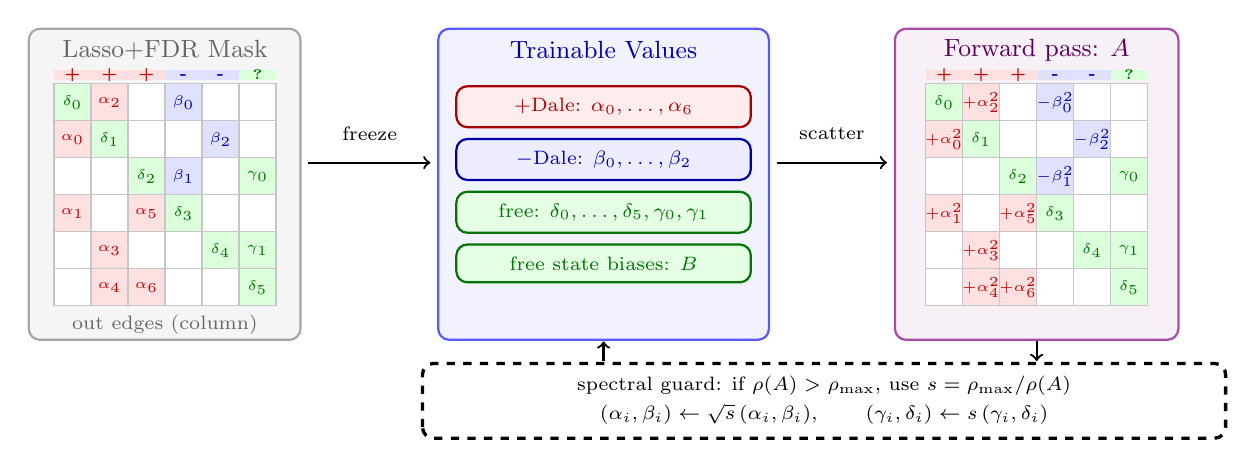
\begin{tikzpicture}[x=1cm,y=1cm]
  % Stage B aggregate input
  \draw[rounded corners, thick, gray!70, fill=gray!8] (0.55,1.10) rectangle (4.00,5.05);
  \node[gray!80!black] at (2.28,4.78) {\small Lasso+FDR Mask};

  \begin{scope}[shift={(0.87,4.35)}, x=0.47cm, y=0.47cm]
    \foreach \c in {0,1,2} {
      \fill[red!12] (\c,0.10) rectangle ++(1,0.28);
      \node[red!75!black] at (\c+0.5,0.24) {\tiny\bfseries +};
    }
    \foreach \c in {3,4} {
      \fill[blue!12] (\c,0.10) rectangle ++(1,0.28);
      \node[blue!70!black] at (\c+0.5,0.24) {\tiny\bfseries -};
    }
    \fill[green!14] (5,0.10) rectangle ++(1,0.28);
    \node[green!45!black] at (5.5,0.24) {\tiny\bfseries ?};

    \foreach \r in {0,1,2,3,4,5} {
      \foreach \c in {0,1,2,3,4,5} {
        \draw[gray!45, fill=white] (\c,-\r) rectangle ++(1,-1);
      }
    }
    \foreach \k in {0,1,2,3,4,5} {
      \fill[green!14] (\k,-\k) rectangle ++(1,-1);
      \node[green!45!black] at (\k+0.5,-\k-0.5) {\tiny \(\delta_{\k}\)};
    }
    \foreach \r/\c/\lab in {
      1/0/\alpha_0, 3/0/\alpha_1,
      0/1/\alpha_2, 4/1/\alpha_3, 5/1/\alpha_4,
      3/2/\alpha_5, 5/2/\alpha_6} {
      \fill[red!12] (\c,-\r) rectangle ++(1,-1);
      \node[red!75!black] at (\c+0.5,-\r-0.5) {\tiny \(\lab\)};
    }
    \foreach \r/\c/\lab in {0/3/\beta_0, 2/3/\beta_1, 1/4/\beta_2} {
      \fill[blue!12] (\c,-\r) rectangle ++(1,-1);
      \node[blue!70!black] at (\c+0.5,-\r-0.5) {\tiny \(\lab\)};
    }
    \foreach \r/\c/\lab in {2/5/\gamma_0, 4/5/\gamma_1} {
      \fill[green!14] (\c,-\r) rectangle ++(1,-1);
      \node[green!45!black] at (\c+0.5,-\r-0.5) {\tiny \(\lab\)};
    }
    \foreach \r in {0,1,2,3,4,5} {
      \foreach \c in {0,1,2,3,4,5} {
        \draw[gray!45] (\c,-\r) rectangle ++(1,-1);
      }
    }
  \end{scope}
  \node[gray!80!black] at (2.28,1.29) {\scriptsize out edges (column)};

  % Active parameterization
  \draw[->, thick] (4.10,3.35) -- (5.65,3.35);
  \node at (4.88,3.72) {\scriptsize freeze};
  \draw[rounded corners, thick, blue!65, fill=blue!5] (5.75,1.10) rectangle (9.95,5.05);
  \node[blue!65!black] at (7.85,4.78) {\small Trainable Values};

  \draw[rounded corners, thick, red!65!black, fill=red!7] (5.98,3.80) rectangle (9.72,4.32);
  \node[red!70!black, align=center] at (7.85,4.06)
    {\scriptsize \(+\)Dale: \(\alpha_0,\ldots,\alpha_6\)};
  \draw[rounded corners, thick, blue!65!black, fill=blue!7] (5.98,3.13) rectangle (9.72,3.65);
  \node[blue!70!black, align=center] at (7.85,3.39)
    {\scriptsize \(-\)Dale: \(\beta_0,\ldots,\beta_2\)};
  \draw[rounded corners, thick, green!45!black, fill=green!10] (5.98,2.46) rectangle (9.72,2.98);
  \node[green!45!black, align=center] at (7.85,2.72)
    {\scriptsize free: \(\delta_0,\ldots,\delta_5,\gamma_0,\gamma_1\)};
  \draw[rounded corners, thick, green!45!black, fill=green!10] (5.98,1.83) rectangle (9.72,2.31);
  \node[green!45!black, align=center] at (7.85,2.07)
    {\scriptsize free state biases: \(B\)};

  % Forward pass and objective
  \draw[->, thick] (10.05,3.35) -- (11.45,3.35);
  \node at (10.75,3.72) {\scriptsize scatter};
  \draw[rounded corners, thick, violet!70, fill=violet!6] (11.55,1.10) rectangle (15.15,5.05);
  \node[violet!70!black] at (13.35,4.78) {\small Forward pass: \(A\)};

  \begin{scope}[shift={(11.94,4.35)}, x=0.47cm, y=0.47cm]
    \foreach \c in {0,1,2} {
      \fill[red!12] (\c,0.10) rectangle ++(1,0.28);
      \node[red!75!black] at (\c+0.5,0.24) {\tiny\bfseries +};
    }
    \foreach \c in {3,4} {
      \fill[blue!12] (\c,0.10) rectangle ++(1,0.28);
      \node[blue!70!black] at (\c+0.5,0.24) {\tiny\bfseries -};
    }
    \fill[green!14] (5,0.10) rectangle ++(1,0.28);
    \node[green!45!black] at (5.5,0.24) {\tiny\bfseries ?};

    \foreach \r in {0,1,2,3,4,5} {
      \foreach \c in {0,1,2,3,4,5} {
        \draw[gray!45, fill=white] (\c,-\r) rectangle ++(1,-1);
      }
    }
    \foreach \k in {0,1,2,3,4,5} {
      \fill[green!14] (\k,-\k) rectangle ++(1,-1);
      \node[green!45!black] at (\k+0.5,-\k-0.5) {\tiny \(\delta_{\k}\)};
    }
    \foreach \r/\c/\lab in {
      1/0/\alpha_0, 3/0/\alpha_1,
      0/1/\alpha_2, 4/1/\alpha_3, 5/1/\alpha_4,
      3/2/\alpha_5, 5/2/\alpha_6} {
      \fill[red!12] (\c,-\r) rectangle ++(1,-1);
      \node[red!75!black] at (\c+0.5,-\r-0.5) {\tiny \(+\lab^2\)};
    }
    \foreach \r/\c/\lab in {0/3/\beta_0, 2/3/\beta_1, 1/4/\beta_2} {
      \fill[blue!12] (\c,-\r) rectangle ++(1,-1);
      \node[blue!70!black] at (\c+0.5,-\r-0.5) {\tiny \(-\lab^2\)};
    }
    \foreach \r/\c/\lab in {2/5/\gamma_0, 4/5/\gamma_1} {
      \fill[green!14] (\c,-\r) rectangle ++(1,-1);
      \node[green!45!black] at (\c+0.5,-\r-0.5) {\tiny \(\lab\)};
    }
    \foreach \r in {0,1,2,3,4,5} {
      \foreach \c in {0,1,2,3,4,5} {
        \draw[gray!45] (\c,-\r) rectangle ++(1,-1);
      }
    }
  \end{scope}

  % Spectral projection feedback
  \draw[rounded corners, dashed, very thick, black, fill=white]
    (5.55,-0.15) rectangle (15.75,0.80);
  \node[black, align=center] at (10.65,0.33)
    {\scriptsize spectral guard: if \(\rho(A)>\rho_{\max}\), use
     \(s=\rho_{\max}/\rho(A)\)\\[-0.5mm]
     \scriptsize \((\alpha_i,\beta_i)\leftarrow\sqrt{s}\,(\alpha_i,\beta_i),\qquad
     (\gamma_i,\delta_i)\leftarrow s\,(\gamma_i,\delta_i)\)};
  \draw[->, black, thick] (13.35,1.08) -- (13.35,0.83);
  \draw[->, black, thick] (7.85,0.83) -- (7.85,1.08);
\end{tikzpicture}
\caption{Stage (c) de-biased refit cartoon. Stage (b) determines which
off-diagonal edges are allowed to exist and which source columns have fixed
Dale signs. In this toy \(6\times6\) mask, \(\delta_0,\ldots,\delta_5\)
are free diagonal entries, \(\alpha_0,\ldots,\alpha_6\) are edges from
positive Dale columns, \(\beta_0,\ldots,\beta_2\) are edges from negative
Dale columns, and \(\gamma_0,\gamma_1\) are surviving undecided-source
edges. The de-biased trainer carries only active values: \(\alpha_i\) and
\(\beta_i\) for Dale-constrained surviving edges, \(\gamma_i\) for
undecided surviving edges, \(\delta_i\) for all diagonal entries, and \(B\)
for free state biases. Structural zero cells carry no optimizer state. The
forward pass scatters these values into the
effective connectivity matrix \(A\), rebuilds \(A\) for each minibatch,
evaluates the Poisson negative log-likelihood with \(\lambda_3=0\), handles
the states as locked or jointly refit according to the run mode, saves
\texttt{A\_debias} and \texttt{B\_debias}, and applies the spectral-radius
guard in the transformed parameter space.}
\label{fig:stage-c-debias-cartoon}
\end{figure}

% ===============================================================
\section{Methodology: Active-Set Parameter Transformation}
% ===============================================================

To enforce the above constraints without relying on manual clamping (which can disrupt the momentum-based Adam optimizer), we use a parameter transformation for $A$: the \textit{squared-parameter trick}. The complete trainable variable set is $(u,v,B)$: the active connectivity vectors defined below plus the state-bias matrix. The biases are re-fitted jointly with $A$ and are initialized from $\bar{B}$, but they do not need the Dale sign transform. The masks below define the mathematical structure of $A$, but the optimizer should not have to carry full $N\times N$ tensors full of zeros.

We construct two static, mutually exclusive structural masks based on the FDR-bagging output:
\begin{itemize}
    \item $\bm{M_{\text{Dale}}} \in \{-1, 0, 1\}^{N \times N}$: This mask handles off-diagonal surviving edges from signed source nodes. It contains $+1$ for surviving excitatory edges, $-1$ for surviving inhibitory edges, and $0$ otherwise.
    \item $\bm{M_{\text{Free}}} \in \{0, 1\}^{N \times N}$: This mask handles entries whose sign is not Dale-constrained. It contains $1$ for surviving off-diagonal edges from undecided source nodes, $1$ for every diagonal element $A_{ii}$, and $0$ otherwise.
\end{itemize}

The dense mathematical form is
\begin{equation}
\label{eq:dense-transform}
A = \big( M_{\text{Dale}} \odot U^{\circ 2} \big) + \big( M_{\text{Free}} \odot V \big)
\end{equation}
where $\odot$ denotes element-wise multiplication (Hadamard product), and $U^{\circ 2}$ denotes the element-wise square of $U$. This form is useful for reasoning about the constraints. For implementation, however, it is better to fit active vectors:
\begin{equation}
\label{eq:active-index-sets}
\mathcal{D}=\{(i,j):(M_{\text{Dale}})_{ij}\ne0\}, \qquad
\mathcal{F}=\{(i,j):(M_{\text{Free}})_{ij}=1\},
\end{equation}
\begin{equation}
\label{eq:active-vectors}
u\in\mathbb{R}^{|\mathcal{D}|}, \qquad
v\in\mathbb{R}^{|\mathcal{F}|}.
\end{equation}
In each forward pass, initialize $A$ as an all-zero matrix and scatter the active parameters into it:
\begin{equation}
\label{eq:active-scatter}
A_{ij} =
\begin{cases}
    (M_{\text{Dale}})_{ij}\,u_k^2, & (i,j)=\mathcal{D}_k,\\
    v_\ell, & (i,j)=\mathcal{F}_\ell,\\
    0, & \text{otherwise.}
\end{cases}
\end{equation}
Thus each free entry, including every diagonal $A_{ii}$, is copied one-to-one from $v$, while each Dale-constrained edge is generated by squaring the corresponding element of $u$ and applying the fixed sign.

\textbf{Why this works:}
Because $u$ is squared, $u_k^2$ is non-negative. Multiplying it by the sign stored in $M_{\text{Dale}}$ enforces excitatory or inhibitory signs by construction. Meanwhile, the unconstrained vector $v$ allows undecided off-diagonal edges and diagonal self-history terms to explore positive or negative values freely. The vector formulation is also cleaner numerically: pruned edges have no optimizer state, receive no stale momentum, and cannot accidentally re-enter through implementation mistakes.

% ===============================================================
\section{Fitting Details and Safeguards}
% ===============================================================

\subsection{Vanishing Gradients and Initialization}

The primary pitfall of the squared-parameter trick lies in the chain rule of backpropagation. The gradient of the loss $\mathcal{L}$ with respect to a parameter $U_{ij}$ is:
\begin{equation}
\label{eq:dense-u-gradient}
\frac{\partial \mathcal{L}}{\partial U_{ij}} = \frac{\partial \mathcal{L}}{\partial A_{ij}} \cdot 2 U_{ij} \cdot (M_{\text{Dale}})_{ij}
\end{equation}
In the active-vector notation this becomes
\begin{equation}
\label{eq:active-u-gradient}
\frac{\partial \mathcal{L}}{\partial u_k}
= \frac{\partial \mathcal{L}}{\partial A_{ij}} \cdot 2u_k\cdot (M_{\text{Dale}})_{ij},
\qquad (i,j)=\mathcal{D}_k .
\end{equation}
If the optimizer pushes $u_k$ to exactly zero, or initializes it very close to zero, the gradient vanishes entirely. The parameter becomes ``stuck'' and cannot recover, effectively acting as an unintended structural pruning.

\textbf{Mitigation via Initialization:}
To prevent vanishing gradients, initialize the learnable signed-edge parameters securely away from zero, using the approximate shrunk values ($\bar{A}$) from the FDR-bagging stage.
\begin{equation}
\label{eq:active-init}
\begin{aligned}
u_k^{\text{init}} &= \max\!\left(\sqrt{\big| \bar{A}_{ij} \big|},\ \epsilon_u\right),
&\qquad (i,j)&=\mathcal{D}_k,\\
v_\ell^{\text{init}} &= \bar{A}_{ij},
&\qquad (i,j)&=\mathcal{F}_\ell .
\end{aligned}
\end{equation}
Here $\epsilon_u$ is a small positive floor used only for Dale-constrained parameters whose bagged estimate is extremely close to zero. The bias vectors are initialized directly as $B^{\text{init}} = \bar{B}$.

\subsection{Spectral-Radius Projection}

To maintain numerical stability in the Poisson GLM, the effective matrix $A$ must not exceed a maximum spectral radius $\rho_{\text{max}}$ (typically 0.95).

In a standard network, one applies a scalar scaling factor to $A$. In our transformed parameter space, we must apply the scaling to the underlying learnable variables $u$ and $v$ such that the resulting effective $A$ is correctly scaled.

At the configured spectral-projection interval during the M-step, we construct the effective $A$ and calculate its spectral radius $\rho(A)$. If $\rho(A) > \rho_{\text{max}}$, we define a scaling factor:
\begin{equation}
\label{eq:spectral-scale}
\begin{aligned}
\gamma &= \frac{\rho_{\text{max}}}{\rho(A)},\\
u &\leftarrow u \cdot \sqrt{\gamma},\\
v &\leftarrow v \cdot \gamma .
\end{aligned}
\end{equation}
We then update the underlying active parameters \textit{in-place} according to Eq.~\eqref{eq:spectral-scale}.
Because the forward pass squares $u$, scaling $u$ by $\sqrt{\gamma}$ correctly results in the corresponding effective Dale-constrained elements of $A$ being scaled by exactly $\gamma$. Scaling $v$ by $\gamma$ does the same for free entries. Structural zeros are unaffected, diagonal terms remain free, and biological signs cannot flip. The spectral constraint is therefore compatible with the sign constraints, although it can still limit final magnitudes when the unconstrained MLE wants a matrix outside the stable region.

% ===============================================================
\section{Implementation Plan for \texttt{prism\_deBiasFit3c.py}}
% ===============================================================

The production implementation should be a PyTorch distributed trainer, launched
the same way as the existing Stage (a) and Stage (b) jobs:
\begin{verbatim}
module load pytorch
torchrun --standalone --nnodes=1 --nproc_per_node=4 \
  ./prism_deBiasFit3c.py \
  --basePath <basePath> \
  --fdrFitName <stageB_aggregate_name> \
  --outFitName <stageC_output_name>
\end{verbatim}
On Perlmutter this uses the four A100 GPUs assigned to one node. The script
should reuse distributed utilities from \texttt{PrismEM\_Workhorse3c.py}
(\texttt{init\_distributed}, broadcasts, barriers, seeding, pair loaders,
E-step helpers, simplex projection, and Viterbi decoding). The dense
unconstrained \texttt{SwitchingPoissonGLM}, \texttt{run\_full\_fit}, and
\texttt{run\_locked\_mstep} should not be reused directly because Stage (c)
needs the active-vector parameterization $(u,v,B)$ and no $L_1$ pruning. If
the implementation becomes long, put the Stage (c) model and training loop in
\texttt{PrismDeBias\_Workhorse3c.py}, leaving \texttt{prism\_deBiasFit3c.py}
as the command-line, I/O, and provenance wrapper.

\subsection{Inputs and Initialization}

The primary input is the Stage (b) aggregate fit
\texttt{<basePath>/prismFit/<fdrFitName>.prismEM.npz}. The script should
recover the original spike-file stem and the reference EM fit name from the
existing metadata provenance, rather than asking the user to provide multiple
file names. It should then load the source spikes from
\texttt{spikesData/}, slice the same \texttt{time\_range\_bins}, and verify
that the spike window length matches the Stage (b) \texttt{S\_hat} and
\texttt{c\_hat} arrays.

The Stage (c) support and initialization are:
\begin{itemize}
    \item Use Stage (b) \texttt{selected\_mask} for the off-diagonal support.
    \item Use Stage (b) \texttt{neuron\_type} for Dale-constrained source columns.
    \item Put all diagonal entries into the free set $\mathcal{F}$.
    \item Initialize Dale-constrained magnitudes from Stage (b)
    \texttt{A\_hat}: $u_k=\max(\sqrt{|A_{ij}^{(b)}|},\epsilon_u)$, with the
    sign supplied only by $M_{\text{Dale}}$.
    \item Initialize free off-diagonal entries and all diagonal entries from
    Stage (b) \texttt{A\_hat}: $v_\ell=A_{ij}^{(b)}$.
    \item Initialize the bias matrix from Stage (b) \texttt{B\_hat}.
\end{itemize}
Stage (b) \texttt{A\_prune} must be copied to the output unchanged for
comparison, but it is not the fitted Stage (c) matrix.

\subsection{State Handling}

Expose a three-way command-line option:
\begin{itemize}
    \item \texttt{--state\_mode locked}: keep Stage (b) states fixed and fit only
    $(u,v,B)$.
    \item \texttt{--state\_mode refit}: alternate E-step updates of $c_t$ and
    Viterbi decoding with de-biased M-step updates of $(u,v,B)$.
    \item \texttt{--state\_mode auto}: use \texttt{refit} when
    \texttt{num\_states>1}, otherwise use \texttt{locked}.
\end{itemize}
All M-step minibatches should use destination-bin state labels: $S_t$ for
the lag pair $(Y_{t-1},Y_t)$. This matches the Stage (b) FDR-bagging
convention and the rate model in Eq.~\eqref{eq:model-rate}.

\subsection{Training Hyperparameters}

The script should read defaults from the Stage (b) and reference EM metadata,
but expose the important controls explicitly:
\begin{itemize}
    \item \texttt{--num\_debias\_iters}: outer E/M iterations for
    \texttt{state\_mode refit}.
    \item \texttt{--warmup\_locked\_epochs}: optional fixed-state M-step epochs
    before state refitting starts.
    \item \texttt{--m\_epochs}, \texttt{--batch\_size},
    \texttt{--lr\_mstep}, and \texttt{--lr\_end\_factor}: Adam M-step controls.
    \item \texttt{--pgd\_iter}, \texttt{--lr\_estep}, and \texttt{--lambda2}:
    E-step controls used only when states are refit. The parameter
    \texttt{--lambda2} is the temporal smoothness weight on the soft state
    probabilities,
    \[
        \lambda_2 \sum_t \|c_t-c_{t-1}\|_2^2 .
    \]
    In the projected-gradient E-step this contributes the gradient term
    $2\lambda_2(c_t-c_{t-1})$. Larger values make the inferred state
    probabilities change more slowly over time; smaller values allow more
    rapid state switching. It does not regularize $A$ or $B$ directly. In
    \texttt{state\_mode locked}, the states are copied from Stage (b), the
    E-step is skipped, and \texttt{--lambda2} is effectively irrelevant.
    \item \texttt{--rho\_max}, \texttt{--prescale\_m\_step\_4\_ArhoMax},
    \texttt{--delay\_iter\_4\_ArhoMax}, and
    \texttt{--target\_iter\_4\_ArhoMax}: spectral-radius controls.
    \item \texttt{--eps\_u} and \texttt{--seed}: numerical floor and RNG seed.
\end{itemize}
There is no Stage (c) $L_1$ penalty; record \texttt{lambda3=0} in metadata.

\subsection{Output Schema and Provenance}

The output should be written to
\texttt{<basePath>/prismFit/<outFitName>.prismEM.npz}. Preserve the original
Stage (b) arrays for comparison and add unambiguous Stage (c) arrays:
\begin{itemize}
    \item Keep Stage (b) \texttt{A\_hat}, \texttt{A\_prune}, and
    \texttt{B\_hat} unchanged.
    \item Save the direct Stage (c) fit as \texttt{A\_debias} and
    \texttt{B\_debias}.
    \item Save the original Stage (b) states as \texttt{S\_stageB},
    \texttt{c\_stageB}, and \texttt{S\_stageB\_CL}.
    \item Save final display states as \texttt{S\_hat}, \texttt{c\_hat}, and
    \texttt{S\_hat\_CL}. In locked mode these equal the Stage (b) states; in
    refit mode they are the final Stage (c) states.
    \item Save histories for E-step NLL, M-step loss/NLL, spectral radius,
    spectral correction strength, learning rate, and effective nonzero count.
    \item Save support diagnostics: Dale/free index counts, diagonal count,
    selected-edge count, and optional arrays mapping active-vector entries
    back to $(i,j)$ coordinates.
\end{itemize}
Do not perform a second post-fit pruning pass on \texttt{A\_debias}; the
purpose is to inspect the direct constrained MLE result.

Metadata should continue the existing provenance scheme. Set
\texttt{fit\_type="prismEM\_deBias\_stageC"} and add a
\texttt{deBias\_stageC} block containing the program name, input Stage (b)
file/name, recovered reference EM name, source spike file/name,
\texttt{state\_mode}, support construction rules, initialization rules,
hyperparameters, output name, elapsed time, and the trainable parameter
counts. The top-level \texttt{provenance} dictionary should retain all
Stage (a)/(b) entries and add \texttt{deBias\_stageC\_input},
\texttt{deBias\_stageC\_file}, and \texttt{deBias\_stageC\_outFitName}.

\subsection{Plotting Compatibility}

\texttt{prism\_EM\_eval3c.py} should detect Stage (c) files from
\texttt{fit\_type} or the presence of \texttt{deBias\_stageC}. For Stage (c)
outputs it should use \texttt{A\_debias}/\texttt{B\_debias} as the primary
display matrices and include ``Stage (c) de-biased refit'' in plot titles.
For Stage (b) files it should keep the current behavior and title plots as
``Stage (b) FDR aggregate''. The Stage (c) output should nevertheless retain
all relevant arrays so that a dedicated plotter can be built later without
rerunning the fit.

% ===============================================================
\section{Algorithm Summary for Implementation}
% ===============================================================

An agent tasked with implementing Stage (c) should follow these explicit steps:

\begin{enumerate}
    \item \textbf{Load Data:} Load the Stage (b) aggregate, recover the source
    spike file from provenance, slice the Stage (b) time window, and load
    Stage (b) states and aggregates.
    \item \textbf{Construct Static Masks and Index Sets:} Instantiate constant tensors $M_{\text{Dale}}$ and $M_{\text{Free}}$ based on Stage (b) \texttt{selected\_mask}, \texttt{neuron\_type}, and the diagonal. Put signed off-diagonal surviving edges in $\mathcal{D}$ and put undecided surviving off-diagonal edges plus all diagonal entries in $\mathcal{F}$.
    \item \textbf{Initialize Parameters:}
    \begin{itemize}
        \item $u_k \leftarrow \max(\sqrt{|A^{(b)}_{ij}|},\epsilon_u)$ for $(i,j)=\mathcal{D}_k$ \ (requires gradient)
        \item $v_\ell \leftarrow A^{(b)}_{ij}$ for $(i,j)=\mathcal{F}_\ell$ \ (requires gradient)
        \item $B \leftarrow B^{(b)}$ \ (requires gradient)
    \end{itemize}
    \item \textbf{Training Loop (Minibatch Adam):}
    \begin{itemize}
        \item \textit{Forward Pass:} Construct a zero matrix $A$, scatter $(M_{\text{Dale}})_{ij}u_k^2$ into $(i,j)=\mathcal{D}_k$, and scatter $v_\ell$ into $(i,j)=\mathcal{F}_\ell$.
        \item \textit{State Handling:} In locked mode use Stage (b) destination-bin labels. In refit mode update $c_t$ by the E-step, Viterbi-decode $S_t$, and then use destination-bin labels in the M-step.
        \item \textit{Loss:} Compute negative Poisson log-likelihood using $A$ and $B_{\hat{S}_t}$, with no $L_1$ penalty ($\lambda_3 = 0$).
        \item \textit{Backward Pass:} Call \texttt{loss.backward()} and \texttt{optimizer.step()}.
    \end{itemize}
    \item \textbf{Spectral Projection (End of interval):}
    \begin{itemize}
        \item Construct current effective $A$ under \texttt{torch.no\_grad()}.
        \item Compute $\rho(A)$. If $\rho(A) > \rho_{\text{max}}$, compute $\gamma = \rho_{\text{max}} / \rho(A)$.
        \item In-place multiply $u$ by $\sqrt{\gamma}$ and $v$ by $\gamma$.
    \end{itemize}
    \item \textbf{Save Output:} Once converged, construct the final effective matrix and save it as \texttt{A\_debias}; save the jointly fitted biases as \texttt{B\_debias}. Preserve Stage (b) \texttt{A\_hat}, \texttt{A\_prune}, and \texttt{B\_hat} unchanged for comparison. Do not run a second pruning pass on \texttt{A\_debias}.
\end{enumerate}

\end{document}
